\section{Netzwerk Interface}

\begin{figure}[H]
  \begin{center}
    {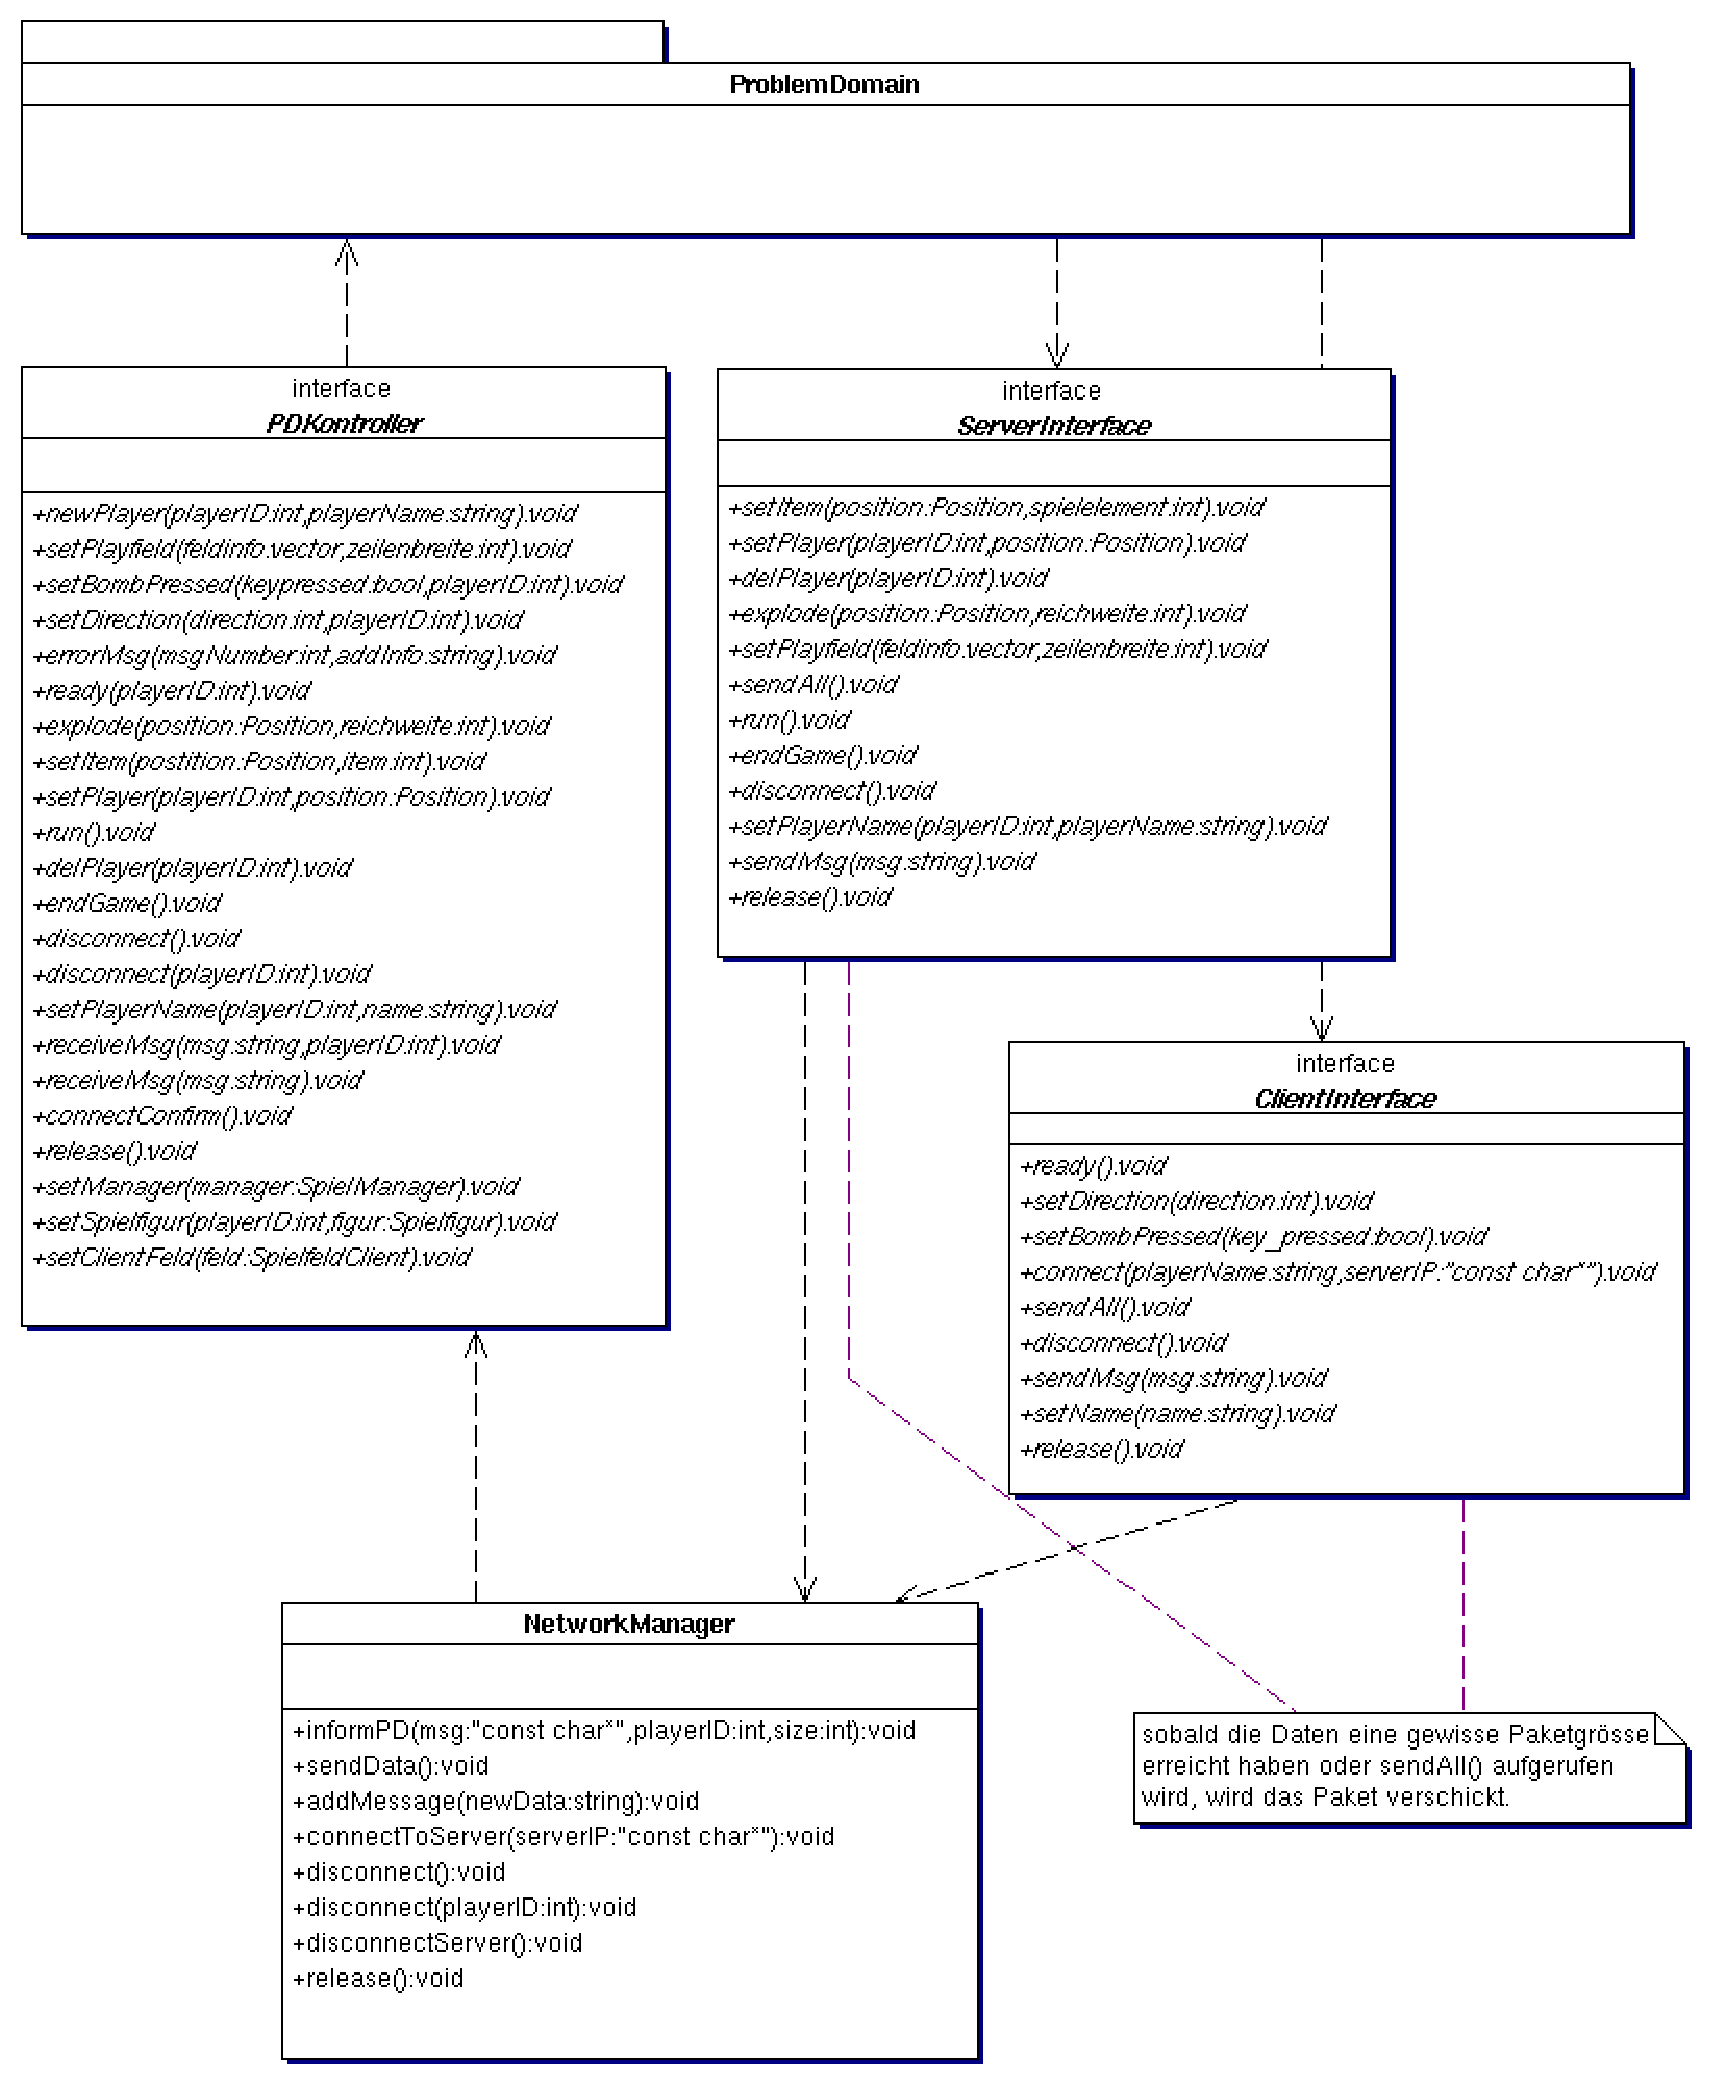
\includegraphics[height=20cm]{./images/netinterface.pdf}}
  \end{center}
  \caption{Interface zwischen Problem Domain und Netzwerk}
\end{figure}

Der Problem Domain stehen die als Singleton implementierten Klassen ServerInterface
und Clientinterface zur Verf"ugung. Die Problem Domain eines Servers verwendet ausschliesslich
das ServerInterface, um mit allen mitspielenden Clients zu kommunizieren. \\
Die Problem Domain eines Clients benutzt das ClientInterface, um sich bei dem Spielserver
anzumelden und ihm Ereignisse zu melden.\\
Die Klassen ServerInterface und ClientInterface rufen ihrerseits Methoden 
der Klasse NetworkManager auf, welcher mit dem Netzwerk kommuniziert. 
Der NetworkManager wird von der Netzwerkschicht aufgerufen und ruft selbst Methoden aus
der Klasse PDKontroller auf.\\
Die Schnittstelle generiert einen tempor"aren String der verschiedene Protokollmessages 
enth"alt. Welche Protokollmessages eingepackt werden ist davon abh"angig, welche Methoden
des Serverinterfaces oder des Clientinterfaces aufgerufen wurden.\\
Dieses Paket wird abgeschickt, sobald es eine gewisse L"ange erreicht hat, oder die Problem Domain
dies durch einen Methodenaufruf ausl"ost.

\section{Netzwerk Interface Klassenbeschreibung}

Verwendete Konstante aus global.h zur Konfiguration des Verhaltens der Schnittstelle:
\\MAX\_STRING\_PAKET\_SIZE. "Ubersteigt der tempor"ar angelegte String der die Nutzdaten 
enth"alt diese L"ange, wird er nach dem Einpacken der letzten Protokollmessage automatisch
verschickt. Zum sofortigen Versenden der Daten kann sowohl im Serverinterface als auch im
Clientinterface die Methode sendAll() aufgerufen werden.
Als Singleton enth"alt diese Klasse auch eine Methode getServerInterface die einen Pointer
auf die Schnittstelle zur"uckgibt.

\subsection{Klasse ServerInterface}
Diese Klasse wird von der Problem Domain des Spielservers benutzt, um Informationen an alle
Spielclients zu schicken. 
Sie ist nach dem Singleton Pattern implementiert.

\subsubsection{Funktionen}
\begin{tabular}{p{50mm}p{90mm}}
+setItem(Position \_pos,int spielelement):void 		 &ein einzelnes Spielelement wird platziert\\
+setPlayer(int playerID, Position \_pos):void 		 &die Spielfigur eines Spielers wird plaziert\\
+delPlayer(int playerID):void;				 &ein Spieler wird aus dem Spiel entfernt\\
+explode(Position \_pos,int reichweite):void		 &signalisiert den Spielclients das Explodieren einer Bombe\\
+setPlayfield(vector$<$int$>$ feldinfo,int zeilenbreite):void&verschickt Spielfelddaten; feldinfo enth"alt Spielelemente;
							  zeilenbreite gibt die Anzahl Felder in einer Horizontalen
							  des Spielfeldes an\\
+sendAll():void 				 	 &l"ost das Versenden des zusammengesetzten Datenpaketes aus\\
+getServerInterface(): ServerInterface*		         &gibt eine Instanz des Serverinterfaces zur"uck\\
+run():void &Startet das Spiel auf den Clients\\
+endGame():void &Signalisiert den Clients das Spielende\\
+disconnect():void&Meldet den Server bei den Clients ab\\
+setPlayerName(int playerID,string playerName):void&Informiert die Clients "uber den Namen eines Spielers\\
+sendMsg(string msg):void&Verschickt an alle Clients eine Nachricht\\
+release():void&l"oscht den Singleton, wenn es keine Referenzen mehr darauf gibt\\
\end{tabular}

\subsection{Klasse ClientInterface}
Das Clientinterface wird von der Problem Domain des Spielclients benutzt, um
Informationen an den Server zu schicken. Sie ist nach dem Singleton Pattern
implementiert.
Als Singleton enth"alt diese Klasse auch eine Methode getClientInterface die einen Pointer
auf die Schnittstelle zur"uckgibt.

\subsubsection{Funktionen}
\begin{tabular}{p{50mm}p{90mm}}
+ready():void 		 &Spielclient meldet sich bereit\\
+setDirection(int direciton):void 		 &Der Server wird "uber die Ausrichtung der Figur informiert\\
+setBombPressed(bool key\_pressed):void;				 &Signalisiert, dass der Spieler Bomben legt\\
+connect(string playerName, const char* serverIP):void		 &Nimmt eine Verbindung zum Spielserver auf\\
+setName(string player\_name):void&Setzt auf dem Server den Spielernamen\\
+sendAll():void 				 	 &l"ost das Versenden des zusammengesetzten Datenpaketes aus\\
+getClientInterface(): ClientInterface*&gibt eine Instanz des Clientinterfaces zur"uck\\
+release():void&l"oscht den Singleton, wenn es keine Referenzen darauf mehr gibt\\
+disconnect():void&Meldet den Client beim Server ab\\
+sendMsg(string msg):void&f"ugt dem tempor"aren Nachrichtenpaket(siehe \ref{Nachrichtenpaket})
 eine Nachricht(siehe \ref{Nachricht}) hinzu\\
\end{tabular}


\subsection{Klasse NetworkManager}
Der NetworkManager wird vom ClientInterface und dem ServerInterface verwendet, um
mit dem Netzwerk zu interagieren. Er speichert die zu versendenden Nachrichten
bis das Nachrichtenpaket eine gewisse Gr"osse hat (s.h. Nachrichtenpaket) oder
dies von einem Interface verlangt wird.\\
Er erh"alt "ubers Netzwerk Nachrichtenpakete und wertet sie aus. Die erhaltene
Information verwendet er um entsprechende Methoden im PDKontroller aufzurufen.
Als Singleton enth"alt diese Klasse auch eine Methode getNetwrokManager die einen Pointer
auf die Schnittstelle zur"uckgibt.

\subsubsection{Funktionen}
\begin{tabular}{p{50mm}p{90mm}}
+getNetworkManager(): NetworkManager*&gibt eine Instanz des NetworkManagers zur"uck\\
+sendData():void&verschickt das zusammengesetzte Nachrichtenpaket(siehe \ref{Nachrichtenpaket}) an den Server\\
+sendServerData():void&verschickt das zusammengesetzte Nachrichtenpaket(siehe \ref{Nachrichtenpaket}) an alle Clients\\
+addMessage(string newData):void&f"ugt dem Nachrichtenpaket(siehe \ref{Nachrichtenpaket}) eine Nachricht (siehe \ref{Nachricht})
	hinzu\\
+informPD(const char* msg,int playerID,int size):void&interpretiert das Nachrichtenpaket(siehe \ref{Nachrichtenpaket}) und ruft die
  entsprechenden Methoden in der Klasse PDKontroller auf\\
+connectToServer(const char* serverIP):void&stellt eine Verbindung zum Server her\\
+release():void&l"oscht den Singleton, wenn es keine Referenz mehr darauf gibt\\
+disconnect():void&Meldet den Client beim Server ab\\
+disconnect(int playerID):void&informiert die PD, falls ein Client nicht mehr erreicht werden kann \\
+disconnectServer():void&ist eine bereitgestellte Methode f"ur das Abmelden des Servers\\
\end{tabular}


\subsection{Klasse StringConverter}
Der StringConverter ist eine Klasse die vom ServerInterface und dem ClientInterface
benutzt wird um Nachrichtencodes und -daten in Pakete zu packen.\\
Der NetworkManager verwendet diese Klasse, um die Nachrichtenpakete wieder
auszupacken und zu interpretieren. Dabei werden Zahlenwerte in Hexadezimalzahlen umgewandelt.

\subsection{Netzwerkprotokoll}
Die Kommunikation zwischen Server und Clients geschieht durch den Austausch von Nachrichtenpaketen
, die verschiedene Nachrichten enthalten k"onnen. Jede Nachricht enth"alt zur Identifikation einen Nachrichtencode.
\subsection{Nachricht}
\label{Nachricht}
Eine Nachricht besteht aus einem Nachrichtencode(siehe \ref{Nachrichtencode}) und einem Datenstring.
\subsubsection{Nachrichtencodes}
\label{Nachrichtencode}
Die Nachrichtencodes charakterisieren den Typ einer Nachricht. Dieser Typ dient dem NetworkManager
zur Identifikation der Methoden und dem Format der Nachrichtendaten. Er wertet die Nachricht aus und ruft
die entsprechende Methode mit den entsprechenden Parametern im PDKontroller auf.\\
\\
In der Datei global.h sind folgende Nachrichten Codes definiert:

\begin {tabular}{p{50mm}p{90mm}}
SET\_ITEM       & = 0\\
SET\_PLAYER     & = 1\\
DEL\_PLAYER     & = 2\\
EXPLODE        & = 3\\
SET\_PLAYFIELD  & = 4\\
REGISTER\_PLAYER& = 5\\
READY          & = 6\\
SET\_DIRECTION  & = 7\\
SET\_BOMB\_KEY   & = 8\\
SET\_NAME       & = 9\\
END\_GAME       & = 10\\
RUN            & = 11\\
DISCONNECT\_SERVER & = 12\\
DISCONNECT\_CLIENT & = 13\\
\end{tabular}
\subsection{Nachrichtenpaket}
\label{Nachrichtenpaket}
Ein Nachrichtenpaket ist ein aus verschiedenen Nachrichten zusammengesetzter String. Eine einzelne Nachricht
besteht aus einem Nachrichtencode und Daten. Es gibt aber auch Nachrichtentypen ohne zus"atzliche Daten.


